\adparagraph{Adjusted nDCG}
In Figure \ref{fig:andcg} we see the scores of the adjusted nDCG measure. All methods generally have high levels of satisfaction according to the measure, with none scoring below 95 percent satisfaction.

Avg is ahead, but it is also the only method using the average rating of all the candidate items for its recommendation.

BC, MC, and SF see a slight increase in score from 16 to 20, which is a curious result.
\begin{figure}[H]
	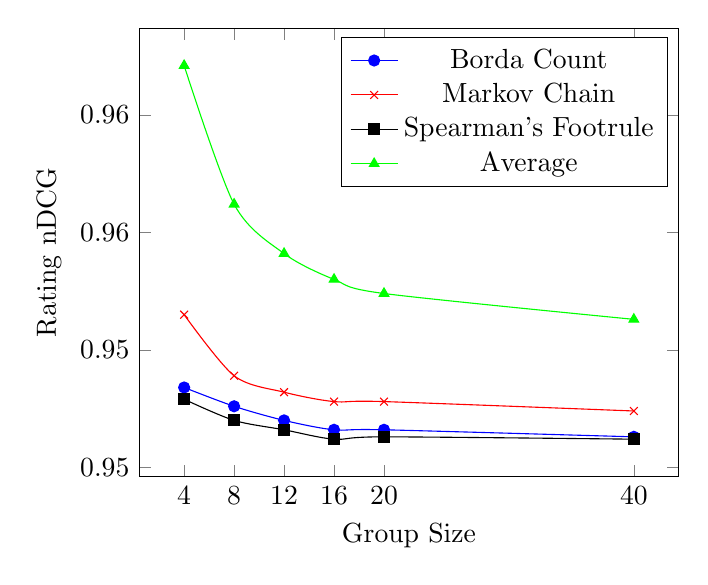
\begin{tikzpicture}
	\begin{axis}[
	xlabel=Group Size,
	ylabel=Rating nDCG,
	xtick = {4,8,12,16,20,40}]
	\addplot[smooth,mark=*,blue] plot coordinates {
		(4,0.9534)
		(8,0.9526)
		(12,0.952)
		(16,0.9516)
		(20,0.9516)
		(40,0.9513)
	};
	\addlegendentry{Borda Count}
	
	\addplot[smooth,color=red,mark=x] plot coordinates {
		(4,0.9565)
		(8,0.9539)
		(12,0.9532)
		(16,0.9528)
		(20,0.9528)
		(40,0.9524)
	};
	\addlegendentry{Markov Chain}
	
	\addplot[smooth,color=black,mark=square*] plot coordinates {
		(4,0.9529)
		(8,0.952)
		(12,0.9516)
		(16,0.9512)
		(20,0.9513)
		(40,0.9512)
	};
	\addlegendentry{Spearman's Footrule}
	
	\addplot[smooth,color=green,mark=triangle*] plot coordinates {
		(4,0.9671)
		(8,0.9612)
		(12,0.9591)
		(16,0.958)
		(20,0.9574)
		(40,0.9563)
	};
	\addlegendentry{Average}
	
	\end{axis}
	\end{tikzpicture}
	\caption{Results for adjusted nDCG test}\label{fig:andcg}
\end{figure}